% !TEX program = pdflatex
% !TEX encoding = UTF-8 Unicode

% Plantilla de la clase `scrbook` del paquete KOMA-script para la
% elaboración de un TFG siguiendo las directrices del la comisión del
% Grado en Matemáticas de la Universidad de Granada.

% Francisco Torralbo Torralbo
% miércoles, 29 de abril de 2020

\documentclass{scrbook}

\KOMAoptions{%
  fontsize=10pt,        % Tamaño de fuente
  paper=a4,             % Tamaño del papel
  headings=normal,      % Tamaño de letra para los títulos: small, normal, big
  % parskip=half,         % Espacio entre párrafos: full (una línea) o half (media línea)
  headsepline=false,    % Una linea separa la cabecera del texto
  cleardoublepage=empty,% No imprime cabecera ni pie en páginas en blanco 
  chapterprefix=false,  % No antepone el texto "capítulo" antes del número
  appendixprefix=false,	% No antepone el texto "Apéndice" antes de la letra
  listof=totoc,		    	% Añade a la tabla de contenidos la lista de tablas y figuras
  index=totoc,			    % Añade a la talba de contenidos una entrada para el índice
  bibliography=totoc,	  % Añade a la tabla de contenidos una entrada para bibliografía
  BCOR=5mm,           % Reserva margen interior para la encuadernación. 
                        % El valor dependerá el tipo de encuadernado y del grosor del libro.
  DIV=10,             % Cálcula el diseño de página según ciertos 
                        % parámetros. Al aumentar el número aumentamos el ancho de texto y disminuimos el ancho del margen. Una opción de 14 producirá márgenes estrechos y texto ancho.
}

% INFORMACIÓN PARA LA VERSIÓN IMPRESA
% Si el documento ha de ser impreso en papel de tamaño a4 pero el tamaño del documento (elegido en \KOMAoptions con la ocpión paper) no es a4 descomentar la línea que carga el paquete `crop` más abajo. El paquete crop se encargará de centrar el documento en un a4 e imprimir unas guías de corte. El procedimiento completo para imprenta sería el siguiente:
% 0. Determinar, según el tipo de encuadernación del documento, el ancho reservado para el proceso de encuadernación (preguntar en la imprenta), es decir, la anchura del área del papel que se pierde durante el proceso de encuadernación. Fijar la varibale BCOR de \KOMAoptions a dicho valor.
% 1. Descomentar la siguiente línea e imprimir una única página con las guías de corte
% 2. Cambiar la opción `cross` por `cam` (o `off`) en el paquete crop y volver a compilar. Imprimir el documento (las guías de corte impresas no inferfieren con el texto).
% 3. Usar la página con las guías impresas en el punto 1 para cortar todas las páginas.

% \usepackage[a4, odd, center, pdflatex, cross]{crop} % Permite imprimir el documento en un a4 (si el tamaño es más pequeño) mostrando unas guías de corte. Útil para imprenta.

% VERSIÓN ELECTRÓNICA PARA TABLETA
% Las opciones siguientes seleccionan un tamaño de impresión similar a una tableta de 9 pulgadas con márgenes estrechos. Útil para producir una versión en pdf para ser leída en una tableta en lugar de impresa.
% Para que la portada quede centrada correctamente hay que editar el
% archivo `portada.tex` y eliminar el entorno `addmargin`

% \KOMAoptions{fontsize=10pt, paper=19.7104cm:14.7828cm, twoside=false, BCOR=0cm, DIV=14}

% ---------------------------------------------------------------------
%	PAQUETES 
% ---------------------------------------------------------------------

% CODIFICACIÓN E IDIOMA
% ---------------------------------------------------------------------
\usepackage[utf8]{inputenc} 			    % Codificación de caracteres

% Selección del idioma: cargamos por defecto inglés y español (aunque este último es el idioma por defecto para el documento). Cuando queramos cambiar de idioma escribiremos:
% \selectlanguage{english} o \selectlanguage{spanish}

\usepackage[english, spanish, es-nodecimaldot, es-noindentfirst, es-tabla]{babel}

% Opciones cargadas para el paquete babel:
  % es-nodecimaldot: No cambia el punto decimal por una coma en modo matemático.
  % es-noindentfirst: No sangra los párrafos tras los títulos.
  % es-tabla: cambia el título del entorno `table` de "Cuadro" a "Tabla"

% Otras opciones del paquete spanish-babel:
  \unaccentedoperators % Desactiva los acentos en los operadores matemáticso (p.e. \lim, \max, ...). Eliminar esta opción si queremos que vayan acentuados

% MATEMÁTICAS
% ---------------------------------------------------------------------
\usepackage{amsmath, amsthm, amssymb} % Paquetes matemáticas
\usepackage{mathtools}                % Añade mejoras a amsmath
\mathtoolsset{showonlyrefs=true}      % sólo se numeran las ecuaciones que se usan
\usepackage[mathscr]{eucal} 					% Proporciona el comando \mathscr para
                                      % fuentes de tipo manuscrito en modo matemático sin sobreescribir el comando \mathcal

% TIPOGRAFÍA 
% ---------------------------------------------------------------------
% El paquete microtype mejora la tipografía del documento.
\usepackage[activate={true,nocompatibility},final,tracking=true,kerning=true,spacing=true,factor=1100,stretch=10,shrink=10]{microtype}

% Las tipografías elegidas para el documento, siguiendo la guía de estilo de la UGR,
% son las siguientes
% Normal font: 			URW Palladio typeface. 
% Sans-serif font: 	Gill Sans
% Monospace font: 	Inconsolata
\usepackage[T1]{fontenc}
\usepackage[sc, osf]{mathpazo} \linespread{1.05}         
\usepackage[scaled=.95,type1]{cabin} % sans serif in style of Gill Sans
% Si el paquete cabin da error usar el siguiente comando en su lugar
% \renewcommand{\sfdefault}{iwona} 
\usepackage{inconsolata}


% Selecciona el tipo de fuente para los títulos (capítulo, sección, subsección) del documento.
\setkomafont{disposition}{\sffamily\bfseries}

% Cambia el ancho de la cita. Al inicio de un capítulo podemos usar el comando \dictum[autor]{cita} para añadir una cita famosa de un autor.
\renewcommand{\dictumwidth}{0.45\textwidth} 

\recalctypearea % Necesario tras definir la tipografía a usar.

% TABLAS, GRÁFICOS Y LISTADOS DE CÓDIGO
% ---------------------------------------------------------------------
\usepackage{booktabs}
% \renewcommand{\arraystretch}{1.5} % Aumenta el espacio vertical entre las filas de un entorno tabular

\usepackage{xcolor, graphicx}
% Carpeta donde buscar los archivos de imagen por defecto
\graphicspath{{img/}}

% IMAGEN DE LA PORTADA
% Existen varias opciones para la imagen de fondo de la portada del TFG. Todas ellas tienen en logotipo de la universidad de Granada en la cabecera. Las opciones son las siguientes:
% 1. portada-ugr y portada-ugr-color: diseño con marca de agua basada en el logo de la UGR (en escala de grises y color).
% 2. portada-ugr-sencilla y portada-ugr-sencilla-color: portada únicamente con el logotipo de la UGR en la cabecera.
\usepackage{eso-pic}
\newcommand\BackgroundPic{%
	\put(0,0){%
		\parbox[b][\paperheight]{\paperwidth}{%
			\vfill
			\centering
      % Indicar la imagen de fondo en el siguiente comando
			
\includegraphics[width=\paperwidth,height=\paperheight,%
			keepaspectratio]{portada-ugr-sencilla}%
			\vfill
}}}

% \usepackage{listings} % Para la inclusión de trozos de código

% CABECERAS
% ---------------------------------------------------------------------
% Si queremos modificar las cabeceras del documento podemos usar el paquete
% `scrlayer-scrpage` de KOMA-Script. Consultar la documentación al respecto.
% \usepackage[automark]{scrlayer-scrpage}

% VARIOS
% ---------------------------------------------------------------------

%\usepackage{showkeys}	% Muestra las etiquetas del documento. Útil para revisar las referencias cruzadas.

% ÍNDICE 
% Para generar el índice hay que compilar el documento con MakeIndex. Generalmente los editores se encargan de ello automáticamente.
% ----------------------------------------------------------------------
% \index{} para añadir un elemento
% \index{main!sub} para añadir un elementos "sub" bajo la categoría "main".
% \index{termino|textbf} para dar formato al número de página (negrita).
% \index{termino|see{termino relacionado}} para crear una referencia cruzada

% Ejemplo: \index{espacio homogéneo}, \index{superficie!mínima}, \index{esfera|see{espacio homogéneo}}

\usepackage{makeidx}
%\usepackage{showidx} % Muestra en el margen del documento las entradas añadidas al índice. Útil para revisar el documento. Si está activo el índice no se genera
\makeindex

% ---------------------------------------------------------------------
% COMANDOS Y ENTORNOS
% ---------------------------------------------------------------------
% Cargamos un archivo externo donde hemos incluido todos los comandos
% propios que vamos a usar en el documento.
% DEFINICIÓN DE COMANDOS Y ENTORNOS

% CONJUNTOS DE NÚMEROS

  \newcommand{\N}{\mathbb{N}}     % Naturales
  \newcommand{\R}{\mathbb{R}}     % Reales
  \newcommand{\Z}{\mathbb{Z}}     % Enteros
  \newcommand{\Q}{\mathbb{Q}}     % Racionales
  \newcommand{\C}{\mathbb{C}}     % Complejos

% TEOREMAS Y ENTORNOS ASOCIADOS

  % \newtheorem{theorem}{Theorem}[chapter]
  \newtheorem*{teora}{Teorema A}
  \newtheorem*{teorb}{Teorema B}
  \newtheorem*{teorema*}{Teorema}
  \newtheorem{teorema}{Teorema}[chapter]
  \newtheorem{proposicion}{Proposición}[chapter]
  \newtheorem{lema}{Lema}[chapter]
  \newtheorem{corolario}{Corolario}[chapter]
  \newtheorem{hecho}{Hecho}[chapter]

    \theoremstyle{definition}
  \newtheorem{definicion}{Definición}[chapter]
  \newtheorem{ejemplo}{Ejemplo}[chapter]

    \theoremstyle{remark}
  \newtheorem{observacion}{Observación}[chapter]


% --------------------------------------------------------------------
% INFORMACIÓN DEL TFG Y EL AUTOR
% --------------------------------------------------------------------
\usepackage{xspace} % Para problemas de espaciado al definir comandos

\newcommand{\miTitulo}{Estructuras diferenciales sobre una superficie topológica y la visualización computacional de superficies.\xspace}
\newcommand{\miNombre}{Norberto Fernández de la Higuera\xspace}
\newcommand{\miGrado}{Doble Grado en Ingeniería Informática y Matemáticas}
\newcommand{\miFacultad}{Facultad de Ciencias}
\newcommand{\miUniversidad}{Universidad de Granada}
% Añadir tantos tutores como sea necesario separando cada uno de ellos
% mediante el comando `\\\medskip` y una línea en blanco
\newcommand{\miTutor}{
  Francisco José López Fernández \\ \emph{Departamento de Geometría y Topología} 

  % Añadir tantos tutores como sea necesario. 
  \medskip
  Carlos Ureña Almagro \\ \emph{Departamento de Lenguajes y Sistemas Informáticos}
}
\newcommand{\miCurso}{2020-2021\xspace}

% HYPERREFERENCES
% --------------------------------------------------------------------
\usepackage{xurl}
\usepackage[pagebackref]{hyperref}
% Opciones para el paquete hyperref
%----------------------------------

\hypersetup{%
  % hidelinks,            % Enlaces sin color ni borde. El borde no se imprime
  linkbordercolor=0.8 0 0,
  citebordercolor=0 0.8 0,
  citebordercolor=0 0.8 0,
  colorlinks = true,            % Color en texto de los enlaces. Comentar esta línea o cambiar `true` por `false` para imprimir el documento.
  linkcolor = [rgb]{0.5, 0, 0}, % Color de los enlaces internos
  urlcolor = [rgb]{0, 0, 0.5},  % Color de los hipervínculos
  citecolor = [rgb]{0, 0.5, 0}, % Color de las referencias bibliográficas
	pdftitle={\miTitulo},%
	pdfauthor={\textcopyright\ \miNombre, \miFacultad, \miUniversidad},%
  pdfsubject={Trabajo de fin de Grado},%
	pdfkeywords={},%
	pdfcreator={pdfLaTeX},%
}

% Redefinición del estilo para mostrar las referencias cruzadas en la bibliografía.
\renewcommand*{\backref}[1]{}
\renewcommand*{\backrefalt}[4]{{\footnotesize [%
    \ifcase #1 No citado%
    \or Citado en pág.~#2%
    \else Citado en págs. #2%
    \fi%
]}}

% Etiquetas en español para el comando \autoref
\def\chapterautorefname{Capítulo}
\def\appendixautorefname{Apéndice}
\def\sectionautorefname{Sección}
\def\subsectionautorefname{Subsección}
\def\figureautorefname{Fig.}
\def\tableautorefname{Tabla}

\def\teoremaautorefname{Teorema}
\def\proposicionautorefname{Proposición}
\def\lemaautorefname{Lema}
\def\corolarioautorefname{Corolario}
\def\definicionautorefname{Def.}
\def\observacionautorefname{Observación}
\def\ejemploautorefname{E.j.}

% Pone automáticamente un parántesis para las ecuaciones
\def\equationautorefname~#1\null{Ec.~(#1)\null}


\begin{document}

% --------------------------------------------------------------------
% FRONTMATTER
% -------------------------------------------------------------------
\frontmatter % Desactiva la numeración de capítulos y usa numeración romana para las páginas

% \pagestyle{plain} % No imprime cabeceras

% !TeX root = ../libro.tex
% !TeX encoding = utf8

%*******************************************************
% Titlepage
%*******************************************************
\begin{titlepage}
  \AddToShipoutPicture*{\BackgroundPic}
  \phantomsection 
  \pdfbookmark[1]{Título}{title}

  % Para que el título esté centrado en la página.
  % Los valores numéricos deberán elegirse de acuerdo con el diseño de
  % página (sobre todo si se cambia la opción BCOR o DIV).
  \begin{addmargin}[2.575cm]{0cm}
  \begin{flushleft}
    \Large  
    \hfill\vfil

    \large{\textsf{\miFacultad}}
    \vfill

    {\large\textsc\miGrado} \vfill


    {\large\textsc{trabajo de fin de grado}}

    \begingroup
    \Huge{\miTitulo}
    \endgroup

    \vfill\vfill\vfill\vfill

    \textsf{\normalsize{Presentado por:}}\\
    {\normalsize\textrm{\miNombre}} 
    \bigskip

    \textsf{\normalsize{Tutor:}}\\
    {\normalsize\rmfamily \miTutor}

    \bigskip
    \textsf{\normalsize{Curso académico \miCurso}}
  \end{flushleft}  
  \end{addmargin}       

\end{titlepage}   
\cleardoublepage
\endinput
                    
% !TeX root = ../libro.tex
% !TeX encoding = utf8

%*******************************************************
% Little Dirty Titlepage
%*******************************************************

\thispagestyle{empty}

\begin{center}
  \large  

  \vspace*{\stretch{1}}

  \begingroup
  \huge{\miTitulo} \\ \bigskip
  \endgroup

  \textrm{\miNombre}

  \vspace{\stretch{5}}

\end{center}  

\newpage
\thispagestyle{empty}

\hfill

\vfill

\miNombre \textit{\miTitulo}.

Trabajo de fin de Grado. Curso académico \miCurso.
\bigskip

\begin{minipage}[t]{0.25\textwidth}
  \flushleft
  \textbf{Responsable de tutorización}
\end{minipage}
\begin{minipage}[t]{0.45\textwidth}
  \flushleft
  \miTutor
\end{minipage}
\begin{minipage}[t]{0.30\textwidth}
  \flushright
  \miGrado
  \medskip

  \miFacultad
  \medskip

  \miUniversidad
\end{minipage}

\newpage
\endinput
                     
% !TeX root = ../libro.tex
% !TeX encoding = utf8
%
%*******************************************************
% Declaración de originalidad
%*******************************************************

\thispagestyle{empty}

\hfill\vfill

\textsc{Declaración de originalidad}\\\bigskip

D./Dña. \miNombre \\\medskip

Declaro explícitamente que el trabajo presentado como Trabajo de Fin de Grado (TFG), correspondiente al curso académico \miCurso, es original, entendida esta, en el sentido de que no ha utilizado para la elaboración del trabajo fuentes sin citarlas debidamente.
\medskip

En Granada a \today 
\begin{flushleft} 
Fdo: \miNombre 

\end{flushleft}

\vfill

\cleardoublepage
\endinput
   
%% !TeX root = ../libro.tex
% !TeX encoding = utf8

%*******************************************************
% Dedication
%*******************************************************
\thispagestyle{empty}
\phantomsection 
\pdfbookmark[1]{Dedicatoria}{Dedicatoria}

\hfill
\vfill

\begin{flushright}
\itshape
Dedicatoria (opcional) \\
Ver archivo \texttt{preliminares/dedicatoria.tex}
\end{flushright}

\vfill

\cleardoublepage
\endinput
                % Opcional
% !TeX root = ../libro.tex
% !TeX encoding = utf8

%*******************************************************
% Table of Contents
%*******************************************************
\phantomsection
\pdfbookmark[0]{\contentsname}{toc}

\setcounter{tocdepth}{2} % <-- 2 includes up to subsections in the ToC
\setcounter{secnumdepth}{3} % <-- 3 numbers up to subsubsections

% \manualmark
% \markboth{\textsc{\contentsname}}{\textsc{\contentsname}}
\tableofcontents 

%*******************************************************
% List of Figures and of the Tables
%*******************************************************

    % *******************************************************
    %  List of Figures
    % *******************************************************    
    \phantomsection 
    \listoffigures

    %*******************************************************
    % List of Tables
    %*******************************************************
    \phantomsection 
    \listoftables
    
    %*******************************************************
    % List of Listings
    % The package \usepackage{listings} is needed
    %*******************************************************      
	  % \phantomsection 
    % \renewcommand{\lstlistlistingname}{Listados de código}
    % \lstlistoflistings 

\cleardoublepage
            
%% !TeX root = ../libro.tex
% !TeX encoding = utf8

%*******************************************************
% Agradecimientos
%*******************************************************

\chapter{Agradecimientos}

Agradezco enormemente el apoyo que he recibido por parte de mi familia y mis dos tutores. Valoro todo el esfuerzo que han realizado por atender mis consultas durante un periodo educativo complicado, sobretodo durante las vacaciones de verano.

\cleardoublepage
\endinput
            % Opcional

% \pagestyle{scrheadings} % A partir de ahora sí imprime cabeceras

% !TeX root = ../libro.tex
% !TeX encoding = utf8
%
%*******************************************************
% Summary
%*******************************************************

\selectlanguage{english}
\chapter{Summary}
This project is about a very important result on differential topology. The main goal is to transmit how complex is the demostration for a student, but been more comprehensible via Allen Hatcher's article \cite{arXiv:1312.3518}. Also, we will translate this problem to the computer scope, showing how difficult is to representate a surface correctly.\\
\\The initial main goals are implement and design an eficient program for visualize homotopies, and demostrate the following theorem as a corollary of the $2$ results cited on Allen Hatcher's article \cite{arXiv:1312.3518}: for all topological manifold exists only one smooth structure, except diffeomorphisms. I have reached both goals and more, because I found some interesting functionalites, like using partials of a defined function on the parametrization, and been able to visualize some characteristics of Morse functions (actually only for ``Height'' function). However, it would have been interesting to have deepened more in Morse theory, but it would have required an exlusive project.\\
\\Initial goals and reached goals.

\section*{Mathematical part}
Mathematical part: previous concepts and results, main results, including corollary.

\section*{Computational part}
Computing part: basic concepts, tessellation study, program structure (processor + visualizer) and used technologies (interface, shaders, optimization).\\

\section*{Conclusions}
These are the key words of the project:
\begin{itemize}
	\item Surface.
	\item Deepen.
	\item Comprehension.
	\item Visualization.
	\item Eficiency.
\end{itemize}

% Al finalizar el resumen en inglés, volvemos a seleccionar el idioma español para el documento
\selectlanguage{spanish} 
\endinput
          
% !TeX root = ../libro.tex
% !TeX encoding = utf8
%
%*******************************************************
% Resumen
%*******************************************************

%\selectlanguage{spanish}
\chapter{Resumen}
El trabajo realizado consiste en el desarrollo de una demostración más sencilla de un teorema clásico de la topología diferencial. Está orientado a transmitir al lector la importancia de dicho resultado. Además, se traslada al ámbito informático para entender la dificultad que colleva representar correctamente una superficie.\\
\\En la parte matemática se trata la demostración de $2$ resultados indicados en el artículo de Allen Hatcher \cite{arXiv:1312.3518} cuyo corolario directo es el teorema central: toda variedad topológica $2$-dimensional tiene una única estructura diferenciable salvo difeormorfismos. Su desarrollo requerirá de mucha información de la teoría de Morse, la cual es muy amplia y por tanto no se aportará un gran nivel de detalle, ya que el objetivo de este proyecto no es la investigación en el campo de dicha teoría.\\
\\La visualización de la superficie se realizará mediante una aproximación con mallas indexadas (conjunto de triángulos), cuyos vértices siempre estarán en la superficie objetivo. El problema residirá en estudiar cuándo es necesario subdividir un triángulo para representar con mayor precisión esa zona.\\
\\Para visualizar correctamente una superficie cualquiera se han estudiado varias definiciones posibles, atendiendo a diferentes cualidades de las superficies. Puesto que lo que se desea es que la superficie se visualize correctamente, la definición escogida estará orientada a cómo la visión humana la percibe. Anque nos centremos en esta definición, trivialmente el límite de la malla indexada será la superficie a representar.\\
\\El estudio de la demostración del teorema nos ha aportado varios recursos bastante interesantes, tales como ``el truco del Toro'' o el uso del grafo asociado a una función de Morse para obtener difeomorfismos de partes de la superficie a discos, anillos, ``pantalones'' o ``pantalones cruzados''.\\
\\Finalmente, el programa implementado nos ha servido de herramienta de visualización de homotopías de manera eficiente, incluso para la función de Morse ``altura'' con dominio la superficie definida. En un futuro se podría incluir la posibilidad de que el usuario indique una función de Morse, pero habría que redefinir los programas ``procesador'' (procesa la parametrización en un lenguaje específico) y ``visualizador'' (visualiza la escena).\\

\newpage
Las palabras clave que definen este proyecto son:
\begin{itemize}
	\item Superficie.
	\item Profundizar.
	\item Entendimiento.
	\item Visualización.
	\item Eficiencia.
\end{itemize}

% Al finalizar el resumen en inglés, volvemos a seleccionar el idioma español para el documento
%\selectlanguage{spanish} 
\endinput

% !TeX root = ../libro.tex
% !TeX encoding = utf8
%
%*******************************************************
% Introducción
%*******************************************************

% \manualmark
% \markboth{\textsc{Introducción}}{\textsc{Introducción}} 

\chapter{Introducción}

En el ámbito matemático, cuando se define una estructura ligada a un elemento, la pregunta natural es si siempre es posible encontrar una para un elemento concreto (existencia) y en caso de que exista, si es la única bajo ciertas condiciones (unicidad).\\
\\Nosotros estudiaremos la existencia y unicidad, salvo difeomorfismos, de una estructura diferenciable para una variedad topológica $2$-dimensional. Este es un teorema clásico de la topología diferencial, cuyas demostraciones previas requieren de un conocimiento amplio en el campo y su realización es extensa. Una de sus demostraciones la realiza James Munkres en su artículo ``Obstructions to Imposing Differentiable Structures'' \cite{Munkres}, aunque él mismo indica en la introducción que S. S. Cairns lo había demostrado para el caso sin borde con la ayuda del teorema de triangulación de E. E. Moise, también indicado en el artículo de Ciprian Manolescu \cite{Historical}.\\
\\Sin embargo, Allen Hatcher en el artículo ``The Kirby Torus Trick for Surfaces'' \cite{arXiv:1312.3518} enuncia y demuestra $2$ resultados cuyo corolario trivial es dicho teorema.\\
\\Cabe destacar que el teorema deja de ser cierto para estructuras de mayor complejidad, como la conforme y la isométrica, he incluso para variedades de dimensión $n \geq 3$.\\
\\Para comprender la importancia del problema de suavizar una ``estructura topológica'', se ha propuesto el estudio de la realización de una buena aproximación a una superficie, gestionando los recursos de manera eficiente para su visualización en tiempo real. Además, permitirá la visualización de homotopías a modo de animaciones fluidas.\\
\\Actualmente estamos observando el auge del hardware para renderizado mediante trazados de rayos, muy útil para la correcta representación de una superficie (bajo un cierto margen de error), pero está lejos de las capacidades de un computador medio si se quiere ejecutar en tiempo real. Es por ello que se ha orientado el estudio al uso de mallas, es decir, aproximar una superficie mediante un conjunto de triángulos, para renderizar mediante rasterizado. El estudio en sí consistirá en detectar en qué zonas será necesaria una mayor cantidad de triángulos para aproximarla mejor.\\
\\Antes de iniciar el estudio del teselado (subdivisión de triángulos) será necesario definir un lenguaje propio para poder indicar explícitamente las cartas de la superficie. Se realizará por medio de un ``procesador'' que dará como salida un código GLSL, que se incluirá en los shaders donde sea necesario. Este programa no funcionará sólo como traductor, sino que tiene el objetivo principal de obtener los árboles de expresión de las funciones definidas y ser capaz de calcular los árboles de las derivadas parciales, para obtener las funciones típicas de una superficie (normal, curvatura, etc).\\
\\Inicialmente se propuso el uso del Geometry shader para implementar un algoritmo de teselado propio, ya que el Geometry shader requiere una versión no muy reciente de OpenGL y aportaría mayor flexibilidad. Sin embargo, por algunas causas que se comentarán en apartado de \textbf{Implementación y pruebas}, decidí utilizar el Tessellation shader, que es más reciente y está diseñado específicamente para el teselado, incrementando considerablemente el rendimiento de la aplicación.\\
\\El problema a tratar es la explicación de la prueba de existencia y unicidad, salvo difeomorfismos, de una estructura diferenciable para toda variedad topológica 2-dimensional sin bordes, de manera que un estudiante del grado de Matemáticas lo entienda con claridad, siempre que suponga ciertos los resultados utilizados de la teoría de Morse. También se diseñará he implementará un programa capaz de visualizar una superficie por cartas, mediante rasterizado, gestionando correctamente los recursos. Además, se ha conseguido incluir la posibilidad de utilizar derivadas parciales de funciones definidas por el ususario y la visualización de funciones de Morse por niveles (isobaras) junto con sus puntos críticos (actualmente sólo para la función de Morse ``altura'').

\section*{Contenido de la memoria}
El trabajo, sin contar las secciones comunes, se ha dividido en $2$ partes, una para la demostración del teorema central (parte matemática) y otra para el estudio de visualización de superficies (parte informática). Cada parte tiene un capítulo dedicado a los conceptos básicos utilizados, para orientar al lector.
\begin{itemize}
	\item Para la parte matemática, el capítulo que trata los conceptos básicos se complementará con otro en el que se indiquen los resultados más importantes utilizados.
	\item En cuanto a la parte informática, se han añadido los capítulos referentes al desarrollo de una aplicación (capítulos 7, 8 y 9), aunque cabe destacar que ha tenido bastante peso el estudio de la teselación, por lo que algunos diagramas no se indicarán si no son relevantes. Es decir, el diseño de la aplicación en sí ha sido el más sencillo posible, para dedicar el mayor tiempo posible a la teselación, eficiencia, robusted y portabilidad de la aplicación.
\end{itemize}
Se han añadido como apéndices una \textbf{Guía de instalación}, donde además se indicarán los requisitos previos, y una \textbf{Guía de uso}.

\section*{Fuentes principales}
Como principales fuentes de información para la realización del proyecto, se han consultado las siguientes referencias:
\begin{itemize}
	\item En la demostración del teorema, los artículos de Allen Hatcher \cite{arXiv:1312.3518} y \cite{MorseTh1}.
	\item Para la implementación del programa, la documentación de OpenGL en la Wiki de Khronos \cite{KhronosWiki} y la de Dear ImGui para la interfaz \cite{ImGui}.
\end{itemize}

\endinput
               

% --------------------------------------------------------------------
% MAINMATTER
% --------------------------------------------------------------------
\mainmatter % activa la numeración de capítulos, resetea la numeración de las páginas y usa números arábigos

\setpartpreamble[c][0.75\linewidth]{%
	\bigskip % Deja un espacio vertical en la parte superior
  Si el trabajo se divide en diferentes partes es posible incluir al inicio de cada una de ellas un breve resumen que indique el contenido de la misma. Esto es opcional.
}
\part{Conocimientos previos} % Dividir un libro en partes OPCIONAL

% !TeX root = ../libro.tex
% !TeX encoding = utf8

\chapter{Variedades topológicas}

\begin{definicion} Una \textbf{variedad topológica} es un espacio de Hausdorff localmente Euclídeo verificando el segundo axioma de numerabilidad, es decir, que su topología tiene una base numerable.
\end{definicion}

Un subconjunto abierto de una variedad es una variedad.

\endinput
%------------------------------------------------------------------------------------
% FIN DEL CAPÍTULO. 
%------------------------------------------------------------------------------------

% !TeX root = ../libro.tex
% !TeX encoding = utf8

\chapter{Estructuras diferenciales}

\section{Resultados previos}

	\begin{teorema} (de ``alisamiento de asas'')
		Sea S una variedad diferenciable, entonces:
		\begin{enumerate}
			\item Un embebimiento $\mathbb{R}^2 \rightarrow S$ puede isotoparse a un embebimiento diferenciable entorno al origen, quedando fijo fuera de un entorno mayor al anterior.
			\item Un embebimiento $D^1\times\mathbb{R} \rightarrow S$ que es diferenciable entorno a $\partial D^1\times\mathbb{R}$ puede isotoparse a un embebimiento diferenciable entorno a $D^1\times 0$, quedando fijo fuera de un entorno mayor al anterior y cercano a $\partial D^1\times\mathbb{R}$.
			\item Un embebimiento $D^2 \rightarrow S$ que es diferenciable entorno a $\partial D^2$ puede isotoparse a un embebimiento diferenciable en todo $D^2$, quedando fijo en un entorno pequeño de $\partial D^2$.
		\end{enumerate}
	\end{teorema}

	\begin{proof}
		Voy a proceder a la demostración de cada uno de los apartados: \\
		\begin{enumerate}
			\item La idea de la demostración es inducir la estructura diferenciable de $S$ ($E_S$) al Toro ($T_S$) , obteniendo así un difeomorfismo de $T_S$ a la estructura diferenciable estándar del Toro (por el \textbf{Hecho 4}), que nos ayudará a construir la isotopía deseada.\\
				\\ Vamos a utilizar el ``truco del toro'', vemos el toro ($T$) como el espacio de órbitas $\mathbb{R}^2/\mathbb{Z}^2$, tomando el $0$ como imagen del $0\in \mathbb{R}^2$. Eliminamos un punto del toro distinto del $0$, y a esta nueva variedad la llamamos $T'$. \\
				\\ Hacemos una inmersión de $T'$ en $\mathbb{R}^2$ manteniendo el $0$ y viendo $T'$ como el interior del disco unidad de $\mathbb{R}^2$ junto con dos 1-asas, que es un embebimiento en el disco (las asas se embeben por separado ya que como se observa, se solapan en $\mathbb{R}^2$ y no es posible hacerlo junto).\\
				\\ Sea $h:\mathbb{R}^2 \rightarrow S$ embebimiento,por el cual $S$ induce una estructura diferenciable en $\mathbb{R}^2$, que denotaremos $E_1$. Por el mismo razonamiento (el embebimiento definido para $T'$), $\mathbb{R}^2$ con la estructura $E_1$ induce una estructura diferenciable en $T'$, que llamaremos $E_2$.\\
				\\ Sabemos por el \textbf{Hecho 3} que existe un conjunto compacto en $T'_{E_2}$ cuyo complemento es difeomorfo a $S^1\times \mathbb{R}$, lo que nos permite extender la estructura diferenciable de $T'$ a $T$, llamada $T_{E_2}$.\\
				\\ Por el \textbf{Hecho 4} sabemos que toda estructura diferenciable del toro ($S^1\times S^1$) es difeomorfa a la estándar. Por tanto, existe un difeomorfismo $g: T_{E_2} \rightarrow T$. Podemos tomar el difeomorfismo $\widehat{g}:\mathbb{R}^2_{E_1} \rightarrow \mathbb{R}^2$ como el levantamiento de la normalización de $g$ (llevar el $0$ en el $0$ y al verlo en $\mathbb{R}^2$ que también deje fijo $\mathbb{Z}^2$ para así poder levantarlo correctamente).\\
				\\ Identificamos $\mathbb{R}^2$ con el interior del disco unidad de $\mathbb{R}^2$ mediante una reparametrización radial que es la identidad entorno al $0$. Entonces tenemos $G:D^2 \rightarrow D^2$ automorfismo en el interior del disco, que tiende a ser también la identidad en el borde (por la condición de que $\|\widehat{g}(x) - x\|$ está acotado para todo $x$, por lo que al tender a infinito las variaciones tienden a $0$, y al reparametrizar $\widehat{g}(x)$ tiende a $x$) y sigue siendo $\widehat{g}$ entorno al $0$. Se puede extender a $G:\mathbb{R}^2 \rightarrow \mathbb{R}^2$, siendo la identidad fuera del interior del disco.\\
				\\ Por el truco de Alexander $G$ es isotópica a la identidad. Se puede obtener la isotopía $G_t$ variando el radio del disco, por lo que cuando el radio tiende a $0$, $G_t$ tiende a ser la identidad ($G_0$). Para $t=1$, $G_1=G$.\\
				\\ Definimos la isotopía para $h$ como $h_t=h\circ G_t^{-1}$, teniendo que $h_0=h$ por ser $G_0$ la identidad. $h_t$ se queda fija fuera del disco unidad ya que $G_t$ es la identidad en dicho conjunto. También tenemos que $h_t(0)=h(0)$ ya que para todo t, $G_t$ es la identidad entorno al $0$. $h_1$ es diferenciable entorno al $0$ respecto a la estructura diferenciable usual de $\mathbb{R}^2$ porque $G_1^{-1}=G^{-1}$ es un difeomorfismo de dicha estructura a $E_1$ entorno al $0$ y $E_1$ es la estructura de $S$ inducida por $h$.
			\item La idea es, al igual que en el punto anterior, encontrar un difeomorfismo entre el dominio de $h$ con diferentes estructuras diferenciables y restringirlo para que esté fijo donde se solicite.\\
				\\ Tenemos $h: D^1\times \mathbb{R} \rightarrow S$ embebimiento diferenciable entorno al borde del dominio. Dicho embebimiento induce una estructura diferenciable en $D^1\times \mathbb{R}$ que al ser $h$ diferenciable entorno al borde, la estructura inducida es igual que la estructura estándar entorno al borde.\\
				\\ Por el \textbf{Hecho 5} tenemos que existe un difeomorfismo $g$ entre la estructura inducida y la estructura estándar de $D^1\times \mathbb{R}$ que es la identidad entorno al borde del conjunto. Tomamos el homeomorfismo $q: D^1\times \mathbb{R} \rightarrow (D^1\times D^1) - (0 \times \partial D^1)$ que es la identidad entorno $D^1\times 0$.\\
				\\ Definimos $G:  (D^1\times D^1) - (0 \times \partial D^1) \rightarrow (D^1\times D^1) - (0 \times \partial D^1)$ por $G = q \circ g \circ q^{-1}$, que como es la identidad entorno al borde del dominio, se puede extender a $G:\mathbb{R}^2 \rightarrow \mathbb{R}^2$. Su comportamiento entorno a $D^1 \times 0$ es igual que $g$ ($q$ es la identidad) y es la identidad fuera de $D^1 \times D^1$ y entorno a $\partial D \times \mathbb{R}$. Podemos tomar $G_t$ la isotopía, de forma que $t$ varía el tamaño del cuadrado $D^1 \times D^1$, de forma similiar a como se hacía en el apartado anterior para el círculo, teniendo así que $G$ es isotópica a la identidad.\\
				\\ Finalmente tomamos la isotopía $h_t = h \circ G_t^{-1}$, con $h_0 = h$ y $h_1$ tal que es $h$ donde $G$ es la identidad y es diferenciable en $D^1 \times 0$ (además de donde ya lo era $h$).
			\item Tenemos $h: D^2 \rightarrow S$ embebimiento que es diferenciable entorno al borde del dominio. Este embebimiento induce una estructura diferenciable de $S$ a $D^2$ que es igual que la estructura diferenciable estándar de $D^2$ entorno al borde, ya que $h$ es diferenciable en dicha zona.\\
				\\ Por el $\textbf{Hecho 6}$ existe un difeomorfismo $g$ entre $D^2$ con la estructura estándar y la inducida, que además es la identidad entorno al borde. El truco de Alexander nos aporta la isotopía $g_t$ donde $t$ va variando el tamaño del disco imagen de $g$ y extendiendo por la identidad, por lo que $g_0$ sería la identidad y $g_1 = g$. Tomando la isotopía $h_t = h \circ g_t^{-1}$ tendríamos lo solicitado, ya que $h_0 = h$ y $h_1$ es igual que $h$ en el borde y es diferenciable en todo el disco.
		\end{enumerate}
		
	\end{proof}
	\begin{corolario}
		El teorema anterior sigue siendo cierto para un abierto de $\mathbb{R}^2$ en vez de para todo $\mathbb{R}^2$.
	\end{corolario}


\section{Hechos utilizados para los teoremas}

\endinput
%------------------------------------------------------------------------------------
% FIN DEL CAPÍTULO. 
%------------------------------------------------------------------------------------

% Añadir tantos capítulos como sea necesario

\cleardoublepage\part{Teorema clásico de Munkres}
% !TeX root = ../libro.tex
% !TeX encoding = utf8

\chapter{Resultados principales}

\section{Enunciados}
	\begin{teora}
		Toda variedad topológica 2-dimensional tiene una estructura diferenciable.
	\end{teora}

	\begin{teorb}
		Todo homeomorfismo entre variedades diferenciables 2-dimensionales es isotópico a un difeomorfismo.
	\end{teorb}
	
	Suponiendo ciertos los teoremas anteriores, es directa la obtención del siguiente resultado, ya que por A tenemos que toda variedad topológica 2-dimensional tiene una estructura diferenciable y por B sabemos que es única salvo difeomorfismos:
	
	\begin{corolario} (Teorema clásico de Munkres)
		Toda variedad topológica 2-dimensional tiene una única estructura diferenciable salvo difeomorfismos.
	\end{corolario}

\section{Demostración del Teorema A}

	\begin{teora}
		Toda variedad topológica tiene una estructura diferenciable.
	\end{teora}
	\begin{proof}[Demostración]
		Sea S una variedad topológica sin borde, podemos coger un sistema coordenado de cartas finito $\{(V_i, h_i)/ 1\leq i\leq N\}$. Vamos a construir por inducción una estuctura diferenciable en el conjunto $U_n = \cup_{i\leq n}h_i(\mathbb{R}^2)$, que por ser un sistema coordenado su límite debe de ser S, probando así el resultado. Cabe destacar que cada $U_i$ contiene a todos los anteriores. \\
		\\ La inducción empieza tomando una carta cualquiera del sistema, $U_1=V_1$ por ejemplo. Si se considera la variedad $U_1$ con el atlas $\{(h_1,U_1)\}$ entonces $h_1$ es diferenciable para ésta de forma trivial (se compone con la inversa y queda la identidad en $\mathbb{R}^2$).\\
		\\ Una vez arrancada la inducción, suponiendo cierto para el paso $n-1$ vamos a extender la diferenciabilidad de $U_{n-1}$ a $U_n$. Sea la carta $(V_n, h_n)$, tomamos entonces $W=h_n^{-1}(U_{n-1})=h_n^{-1}(U_{n-1}\cap h_n(V_n))$, que es un abierto de $\mathbb{R}^2$ por ser $h_n$ un homeomorfismo de $\mathbb{R}^2$ a $V_n$. \\
		\\ Tenemos $W\subset V_n$ abierto en $\mathbb{R}^2$, por el \textbf{Hecho 1} sabemos que existe una triangulación geométrica suya y que al ser abierto (no tiene borde) al ir acercándose al borde los triángulos tienden a ser puntos. Queremos aplicar el ``Teorema de alisamiento de asas'' en los vértices de los triángulos, seguidamente en los lados y finalmente en el interior de cada uno (aplicar los 3 apartados del teorema de forma consecutiva), pero para ello es necesario partir de un embebimiento de $\mathbb{R}^2$:
		\begin{enumerate}
			\item Para cada vértice $p$, elegimos una bola abierta lo suficientemente pequeña de forma que sus cierres no se corten (lo hacemos para todos los vértices de una vez), $B(p,\varepsilon _p)\subset W$ que es difeomorfo a $\mathbb{R}^2$ ($f_p:\mathbb{R}^2\rightarrow B$ difeomorfismo, con $f_p(0)=p$). Tomamos $g=h_n\circ f_p:\mathbb{R}^2\rightarrow h_n(W)$, que es un embebimiento por serlo $h_n|_B:B\rightarrow h_n(W)$ y $f_p$ (la composición de embebimientos es un embebimiento). \\
			\\ Aplicamos el apartado 1 del Teorema de alisamiento de asas y obtenemos una $\widehat{g}$ isotópica a la primera, que es diferenciable en $O_p$ (entorno abierto del origen, con $0=f_p^{-1}(p)$) y además queda fija fuera de otro entorno un poco mayor $O_p'\supset O_p$, con $\overline{f_p(O_p)}\subset B $. Si tomamos la función a trozos $\widehat{h}_n|_{B}=\widehat{g}\circ f_p^{-1}$ y $\widehat{h}_n|_{W-B}=h_n$, está bien definida porque en $B-f_p(O_p)$ al aplicar $f_p^{-1}$ nos lleva a $\mathbb{R}^2-O_p$, que es donde $\widehat{g}=g$, es decir: \\
			\begin{center}
				$\widehat{h}_n|_{B-f_p(O_p)}=\widehat{g}\circ(f_p^{-1}|_{B-f_p(O_p)})=g\circ(f_p^{-1}|_{B-f_p(O_p)})=h_n|_{B-f_p(O_p)}$\\
			\end{center}
			por lo que la función a trozos está bien definida, es diferenciable entorno a $p$ y no se altera fuera de $B$. \\
			\\ Éste paso se puede realizar de forma simultánea para todos los vértices, obteniendo así una $\widehat{h}_n$ que es diferenciable entorno a todos los vértices y se mantiene $h_n$ fuera de un entorno de cada vértice, algo mayor que el anterior (entornos con cierres disjuntos). Es por ello que para no cargar demasiado la notación se llamará a esa nueva función $h_n$.
			\item Tenemos un $h_n$ que es diferenciable entorno a los vértices de los triángulos y queremos usar el apartado 2 del Teorema de alisamiento de asas para extender la diferenciabilidad a un entorno tubular de los lados de los triángulos. Para ello, vemos que en cada lado, junto con los entornos de los vertices, podemos incluir un rectángulo abierto (conjunto abierto de $W$) que contenga a todo el segmento y cuyos segmentos laterales del rectángulo estén contenidos en ambas bolas. Este conjunto es difeomorfo a $\mathbb{R}^2$ y aplicando previamente dicho difeomorfismo cumplimos las hipótesis deseadas.\\
			\\ Al proseguir de forma semejante al apartado anterior, conseguimos una función $h_n$ que es diferenciable en un entorno del conjunto de todos los lados, quedando fija fuera de un entorno algo más grande.
			\item Buscamos finalmente una curva dentro del``esqueleto'' de entornos de los lados de los triángulos que junto con su componente interior sea difeomorfa a la bola cerrada unidad, para aplicar el 3$^{er}$ apartado del Teorema de alisamiento de asas y así obtener una $h_n$ diferenciable en todo $W$.\\
			\\ La curva buscada debe ser diferenciable, cerrada y simple, para así decir que es una curva de Jordan y aplicar el Teorema de la curva de Jordan. Como consecuencia, sabemos que su componente interior es difeomorfa a la bola unidad de $\mathbb{R}^2$. Podemos reducir el problema a buscar dicha curva para el entorno tubular de un triángulo equilátero, ya que es difeomorfo al de un triángulo cualquiera. Además, podemos seguir simplificándolo, aportando únicamente una curva no cerrada cuyos extremos se puedan pegar consecutivamente, siendo infinitamente derivable en los puntos donde se unen.\\
			\\ Haciendo uso de una función meseta $f$ que vale $0$ en $\mathbb{R}^-$ y $1$ a partir de $\epsilon > 0$, si tomamos $g(x)=tg(\frac{\pi}{3})xf(x)$ en el intervalo $[-1,\epsilon]$, tenemos que $g(-1)=0$ y $g(\epsilon)=tg(\frac{\pi}{3})\epsilon$  al igual que sus derivadas, por lo que si vamos alternando $g(x)$ y $g(-x)$ mediante rotaciones y traslaciones, tendremos una curva $\alpha$ diferenciable (suavización del triángulo equilátero). \\
			%\newpage
			\begin{figure}[h]
  				\centering
  				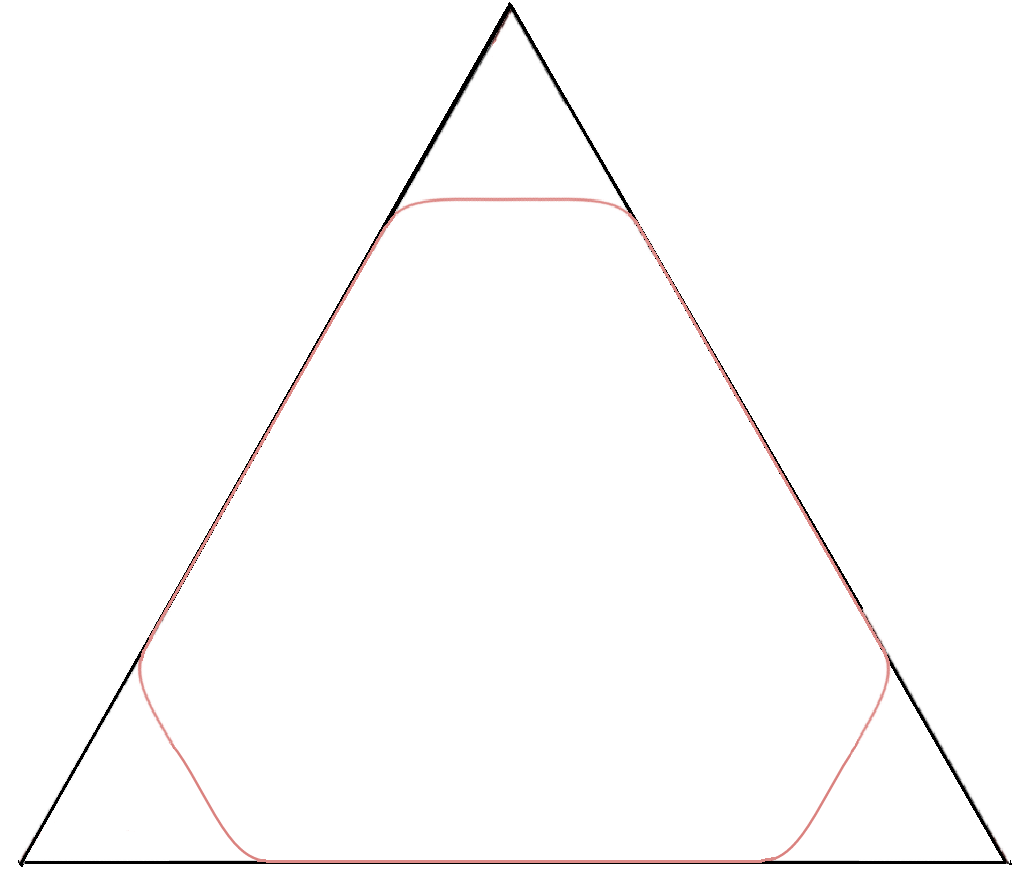
\includegraphics[width=0.5\textwidth]{triangulo_suavizado}
  				\caption{Curva de Jordan cercana al triángulo}
  				\label{fig:triangulo_suavizado}
			\end{figure}
			\\ Se puede observar que es válido $\forall \epsilon > 0$ y que al hacer tender $\epsilon$ a $0$, la curva será el propio triángulo equilátero. Es por ello que podemos tomar el $\epsilon$ lo suficientemente pequeño como para que la curva $\alpha$ quepa en el entorno tubular y siga siendo una curva de Jordan. \\
			\\ Ya tenemos un difeomorfismo entre la bola unidad y la componente interior de cada uno de los triángulos, que contienen un abierto conexo en el cual la función no es todavía diferenciable. Estamos en las condiciones del punto 3 del Teorema de alisamiento de asas, así que procediendo de igual forma que en los apartados anteriores obtenemos una $h_n$ totalmente diferenciable en $W$.
		\end{enumerate}
		
		Cabe destacar que en el borde de $W$ la aplicación se queda intacta, ya queen todo momento se está trabajando en el interior de $W$ (es abierto) y en todo paso de la "suavización" de $h_n$ siempre se deja inalterado el espacio complemento de un entorno mayor al aquel donde se obtiene la diferenciabilidad. Es por ello que se puede extender el $h_n$ obtenido a todo $\mathbb{R}^2$ junto con el original, porque está bien definido, quedando intacta en $\mathbb{R}^2-W$. 
	\end{proof}

\section{Demostración del Teorema B}
	\begin{teorb}
		Todo homeomorfismo entre variedades diferenciables 2-dimensionales es isotópico a un difeomorfismo.
	\end{teorb}
	\begin{proof}[Demostración]
		Sea $f: S \rightarrow S'$ homeomorfismo entre variedades diferenciales 2-dimensionales, se pueden dar 2 casos:
		\begin{enumerate}
			\item $\partial S = \phi$, por lo que podemos utilizar el \textbf{Hecho 2}, que nos aporta una triangulación diferenciable. Si utilizamos el mismo sistema coordenado que para la demostración del Teorema A, al aplicar $h_i^{-1}$ a dicha triangulación diferenciable, por definición tenemos una triangulación clásica en $\mathbb{R}^2$. Si componemos $f$ con $h_i$ ($g=f\circ h_i$), tenemos un embebimiento $g: \mathbb{R}^2 \rightarrow S'$.\\
			\\ Aplicando los apartados del Teorema de alisamiento de asas conseguimos un embebimiento diferenciable $\widehat{g}$ isotópico a $g$, y tomando $\widehat{f}=\widehat{g}\circ h_i^{-1}$ tenemos un homeomorfismo diferenciable isotópico a $g\circ h_i^{-1}=f$. De forma simétrica, aplicándolo a $\widehat{f}^{-1}$, obtenemos que $f$ es isotópico a un difeomorfismo. 
			\item $\partial S \neq \phi$, podemos considerar un collar diferenciable de $\partial S$ en $S$ e isotopar f a a un homeomorfismo diferenciable cerca del borde, dentro de ese conjunto, independientemente del difeomorfismo elegido para el collar diferenciable. Dicha isotopía se obtendrá utilizando el Teorema de alisamiento de asas, tal y como se ha hecho en el apartado anterior. La isotopía dejará fija a $f$ fuera del collar diferenciable. Lo hacemos de igual forma para la inversa, obteniendo una isotopía que deja fija a $f^{-1}$ fuera de un collar diferenciable del borde de $S'$, siendo diferenciable en otro collar diferenciable contenido en el anterior.\\
			\\ Ahora partimos de un homeomorfismo diferenciable en el borde de $S$, aplicando lo utilizado en el apartado anterior podemos obtener una isotopía a $\widehat{f}$, que es un difeomorfismo de $S$ a $S'$,ya que se puede tomar una triangulación en los interiores de las superficies (entendemos por interior a la superficie menos su borde). Aplicamos los mismos pasos para la inversa de $\widehat{f}$, obteniendo así que $f$ es isotópico a un difeomorfismo en todo $S$.
		\end{enumerate}
	\end{proof}
\endinput
%------------------------------------------------------------------------------------
% FIN DEL CAPÍTULO. 
%------------------------------------------------------------------------------------


\cleardoublepage\part{Visualización de superficies}
% !TeX root = ../libro.tex
% !TeX encoding = utf8

\chapter{Segundo capítulo}
\dictum[Leonard Euler]{Mathematicians have tried in vain to this day to discover some order in the sequence of prime numbers, and we have reasons to believe that it is a mystery into which the human mind will never penetrate.}

\section{Primera sección}

\endinput
%------------------------------------------------------------------------------------
% FIN DEL CAPÍTULO. 
%------------------------------------------------------------------------------------


% --------------------------------------------------------------------
% APPENDIX: Opcional
% --------------------------------------------------------------------

\appendix % Reinicia la numeración de los capítulos y usa letras para numerarlos
\pdfbookmark[-1]{Apéndices}{appendix} % Alternativamente podemos agrupar los apéndices con un nuevo \part{Apéndices}

%% !TeX root = ../libro.tex
% !TeX encoding = utf8

\chapter{Primer apéndice}\label{ap:apendice1}

Los apéndices son opcionales.

Archivo: \texttt{apendices/apendice01.tex}

\endinput
%------------------------------------------------------------------------------------
% FIN DEL APÉNDICE. 
%------------------------------------------------------------------------------------

% !TeX root = ../libro.tex
% !TeX encoding = utf8

\chapter{Instalación del software}\label{ap:apendice1}

Los apéndices son opcionales.

Archivo: \texttt{apendices/guia\_instalacion.tex}

\endinput
%------------------------------------------------------------------------------------
% FIN DEL APÉNDICE. 
%------------------------------------------------------------------------------------

% !TeX root = ../libro.tex
% !TeX encoding = utf8

\chapter{Guía de uso del programa}\label{ap:apendice2}

En este capítulo se explicará brevemente cómo utilizar el programa. Aun así, la interfaz del programa se ha intentado diseñar lo más sencilla y clara posible, mostrando adicionalmente cuadros de texto si se mantiene el ratón sobre ciertos elementos.\\
\\Primero iniciaremos el programa tal y como se indica en el apéndice de \textbf{Instalación del software}. Una vez abierto el programa se mostrará siempre la última parametrización compilada existosamente. En el lateral izquierdo aparecerá un elemento de la interfaz, el menú, donde se podrá:
\begin{itemize}
	\item Parametrización:
	\begin{itemize}
		\item Seleccionar una parametrización ya existente, crearla o compilarla. También se podrá editar la actual, en cuyo caso aparecerá una ventana de edición de la propia interfaz. Dicha ventana también aparecerá en caso de que hayan errores léxicos, sintácticos o semánticos en la parametrización, con la salida del error desplegada.
		\item Cambiar el tamaño de la malla de partida, requeriendo su posterior actualización manual (botón contiguo).
		\item Visualizar la ventana con los parámetros temporales, con un tick que indica si está activa la ventana o no. Estará semi-visible si la superficie no tiene parámetros temporales. Dicha ventana mostrará los parámetros temporales en orden, permitiendo moverlos manualmente o generar una animación:
		\begin{itemize}
			\item Sin: movimiento sinusoidal entre el valor $0$ y $1$. Ideal para animaciones oscilantes.
			\item Lineal: movimiento lineal del valor $0$ al $1$, volviendo instantáneamente al $0$. Utilizado para movimientos lineales respecto al tiempo, que junto con el uso de funciones periódicas se puede generar la sensación de movimiento infinito (como los ejemplos wavesX.in).
		\end{itemize}
	\end{itemize}
	\item Visualización del objeto:
	\begin{itemize}
		\item Invertir normales (si no se quiere modificar la parametrización).
		\item Visualizar en modo malla (``Poligon mode'').
		\item Activar/desactivar la auto-rotación (rotación entorno al punto hacia el que mira la cámara).
		\item Ver los vectores tangentes, bitangentes y normales a los puntos (ya sean los de la malla inicial o de todos los generados).
		\item Cambiar modo del color de la superficie, ya sea el color base, la curvatura de Gauss, el área diferencial, la altura o los puntos críticos de ésta vista como función de Morse. Una vez seleccionado un modo, aparecerán coeficientes que permitirán ajustar correctamente la visualización a la superficie actual.
	\end{itemize}
	\item Opciones del teselado:
	\begin{itemize}
		\item Desactivar/activar el teselado.
		\item Indicar la precisión a la que se desea llegar con el teselado.
		\item Opciones avanzadas: modificar aquellos coeficientes específicos del teselado, como el tipo de mejora de rendimiento a usar (``improve'' normal o específica), la distancia de teselado, el umbral para detectar bordes y el exponente aplicado a la curvatura de Gauss. Todos ellos se inician con un valor por defecto.
	\end{itemize}
	\item Iluminación: es posible cambiar los coeficientes del modelo de iluminación ``Phong'' y ver el vector de dirección de la luz actualmente. La luz no es direccional, el vector indica la dirección de la luz con respecto al origen $(0,0)$.
	\item Estadísticas: muestra los fotogramas por segundo y la latencia medias, junto con el número de primitivas generadas tras la fase del geometry shader (después del tessellation shader). Permite además grabar los datos y los almacena de manera automática tras 22 segundos (antes si pulsamos ``Stop'' y seguidamente ``Save info'') en un fichero en el directorio raíz, con nombre dependiente de la parametrización y configuración actual.
\end{itemize}

\endinput
%------------------------------------------------------------------------------------
% FIN DEL APÉNDICE. 
%------------------------------------------------------------------------------------

% Añadir tantos apéndices como sea necesario 

% --------------------------------------------------------------------
% CONCLUSIONES
% --------------------------------------------------------------------

% !TeX root = ../libro.tex
% !TeX encoding = utf8
%
%*******************************************************
% Introducción
%*******************************************************

% \manualmark
% \markboth{\textsc{Introducción}}{\textsc{Introducción}} 

\chapter*{Conclusiones}
\addcontentsline{toc}{chapter}{Conclusiones} % Añade el glosario a la tabla de contenidos

De acuerdo con la comisión de grado, el TFG debe incluir una introducción en la que se describan claramente los objetivos previstos inicialmente en la propuesta de TFG, indicando si han sido o no alcanzados, los antecedentes importantes para el desarrollo, los resultados obtenidos, en su caso y las principales fuentes consultadas.

Ver archivo \texttt{preliminares/conclusiones.tex}

\endinput


% --------------------------------------------------------------------
% GLOSARIO: Opcional
% --------------------------------------------------------------------

% !TeX root = ../libro.tex
% !TeX encoding = utf8

\chapter*{Glosario}
\addcontentsline{toc}{chapter}{Glosario} % Añade el glosario a la tabla de contenidos

La inclusión de un glosario es opcional.

Archivo: \texttt{glosario.tex}

\begin{description} 
  \item[$\mathbb{R}$] Conjunto de números reales.

  \item[$\mathbb{C}$] Conjunto de números complejos.

  \item[$\mathbb{Z}$] Conjunto de números enteros.
\end{description}
\endinput
 

% -------------------------------------------------------------------
% BACKMATTER
% -------------------------------------------------------------------

\backmatter % Desactiva la numeración de los capítulos
\pdfbookmark[-1]{Referencias e Índices}{BM-Referencias}

% BIBLIOGRAFÍA
%-------------------------------------------------------------------

\setbibpreamble{Las referencias se listan por orden alfabético. Aquellas referencias con más de un autor están ordenadas de acuerdo con el primer autor.\par\bigskip}
\bibliographystyle{alpha} 
\begin{small} % Normalmente la bibliografía se imprime en un tamaño de letra más pequeño.
\bibliography{library.bib}
\end{small}


% ÍNDICE TERMINOLÓGICO  (Opcional) 
%------------------------------------------------------------------- 

\cleardoublepage 
\begin{footnotesize} % Normalmente el índice se imprime en un tamaño de letra más pequeño.
\printindex 
\end{footnotesize}

\end{document}
